\chapter{Unsupervised Learning}
\section{Dimensional Reduction and Data Visualization}
\label{sec:dimRed}
In this section, we will begin our foray into unsupervised learning by way of data visualization. Data visualization methods are important for modelling as they can be used to identify correlated or redundant features along with irrelevant features (noise) from raw or processed data. For data involving a relatively small number of features, studying pair-wise correlations (i.e. pairwise scatter plots of all features) may suffice in performing a complete analysis. This rapidly becomes impractical for datasets involving a large number of measured features (such as images). \begin{mybox}{Dimensional Reduction}
	Thus, in practice, we often have to perform \emph{dimensional reduction}, namely, project or embed the data onto a lower dimensional space, which we refer to as the \emph{latent} space.\\
	A recurrent objective of dim. red. techniques is to preserve the relative pairwise distances (or defined similarities) between data points from the original space to the latent space.
\end{mybox}
Part of the complication of dim. red. lies in the fact that low-dimensional representations of high-dimensional data necessarily incurs information loss.

\subsection{Some of the challenges of high-dimensional data}
\label{subsec:dimRedChallengesData}
\subsubsection{High-dimensional data lives near the edge of sample space}
Like one sees in statistical physics, for high-dimensional data, approximately all of the datapoints are contained only in the surface of the $D$-dimensional sphere/cube/... describing it.

\subsubsection{Real-world data vs. uniform distribution}
Fortunately, real-world data is not random or uniformly distributed.\\
In facet, real data usually lives in a much lower dimensional space than the original space in which the features are being measured. This is sometimes referred to as the \emph{blessing of non-uniformity} (in opposition to the curse of dimensionality \ref{subsubsec:performanceevalCurseDimensionality}). 
\begin{example}
	For weakly interacting particles in stat. phys., one can describe them via thermodynamic variables containing the macroscopic dynamics without having to specify the high-dimensional $N\propto 10^{23}$ amount of d.o.f. of the respective phase space dynamics of every particle in the ensemble.
\end{example}

\subsubsection{Intrinsic dimensionality and the crowding problem}
\begin{mybox}{Intrinsic dimensionality of the data}
	Qualitatively, this refers to the minimum number of dimensions (parameters) required to capture the signal in the data (to parametrize the data).  For example, if a data set is described by a sphere, then you need three parameters ($r,\vartheta,\varphi$), i.e. an intrinsic dimensionality of $3$, to parametrize the sphere $S^2 \subset \mR^3$.
\end{mybox}
\begin{mybox}{Crowding problem}
	Attempting to represent data in a space of dimensionality lower than its intrinsic dimensionality can lead to a \emph{crowding problem}. In short, because we are attempting to satisfy too many constraints (e.g. preserve all relative distances of the original space), this results in a trivial solution for the latent space where all mapped data points collapse to the centre of the map. In our example, if you collapse the sphere into two-dimensions, i.e. the circle with variable radius, the two hemispheres would be projected non-bijectively onto the circle, i.e. $\vartheta\in [0,\pi)\mapsto \vartheta=const$. Thus, you would lose a lot of information via the embedding in $\mR^2$.
\end{mybox}
To alleviate this, one needs to weaken the constraints imposed on the visualization scheme. Powerful methods such as t-distributed stochastic embedding (t-SNE) and uniform manifold approximation and projection (UMAP) have been devised to circumvent this issue in various ways.


\subsection{Principal component analysis (PCA)}
\label{subsec:dimRedPCA}
\begin{mybox}{PCA}
A ubiquitous method for dimensional reduction, data visualization and analysis is \emph{Principal Component Analysis} (PCA). The goal of PCA is to perform an orthogonal transformation of the data in order to find high-variance directions. PCA is inspired by the observation that in many cases, the relevant information in a signal is contained in the directions with largest variance. This can be seen as ’fitting’ an ellipse to the data with the major axis corresponding to the first principal component (direction of largest variance).
\end{mybox}
Such PCA-based projections often capture a lot of the large scale structure of many datasets. Even without prior physical knowledge, one can extract relevant order parameters using a simple PCA-based projection.
\subsubsection{The theory}
\label{subsubsec:dimRedPCAtheory}
Consider $N$ data points, $\{\mx_1,\dots,\mx_N\}$ that live in a $p$-dimensional feature space $\mx_i \in \mR^p$. Denote the $N\times p$ design matrix as $\mX = [\mx_1,\dots,\mx_N]^T$ whose rows are the data points and columns correspond to different features, compare \ref{subsec:recipeML}. The $p\times p$ (symmetric) covariance matrix is therefore 
\be 
\label{eq:dimRedPCAcovMatrix}
\mS(\mX) = \frac{1}{N-1} \mX^T \mX.
\ee 
notice that the $j$-th diagonal entry of $\mS(\mX)$ corresponds to the variance of the $j$-th feature and $\mS(\mX)_{ij}$ measures the covariance (i.e. connect correlation in the language of physics) between feature $i$ and feature $j$.\\
Via singular value decomposition (SVD), one finds
\be 
\mS(\mX) = \mathbf{V} \left(\frac{\mathbf{S}^2}{N-1}\right) \mathbf{V}^T \equiv \mathbf{V}\mathbf{Λ} \mathbf{V}^T,
\ee 
where $\mathbf{V}$ contains (as its columns) the right singular vectors of $\mX$, and $\mathbf{Λ}$ is a diagonal matrix with eigenvalues $\lambda_i =s^2_i/(N-1)$ ($s_i$ are the singular values) in the decreasing order along the diagonal (i.e. eigendecomposition). It is clear that the right singular vectors of $\mX$ (i.e. the columns of $\mathbf{V}$) are principal directions of $\mS(\mX)$, and the singular values of $\mX$ are related to the eigenvalues of the covariance matrix $\Sigma(\mX)$ via $\lambda_i$. To reduce the dimensionality of data from $p$ to $\tilde{p}<p$, we first construct the $p\times \tilde{p}$ projection matrix $\mathbf{V}_{\tilde{p}}$ by selecting the singular components with the $\tilde{p}$ largest singular values. The projection of the data from $p$ to $\tilde{p}$ is simply $\tilde{\mathbf{Y}}=\mX \mathbf{V}_{\tilde{p}}$. \\
The singular vector with the largest singular value (i.e. the largest variance) is referred to as the first principal component; the singular vector with the second largest singular value as the second principal component, and so on. An important quantity is the ratio $\lambda_i/\sum_{i=1}^p \lambda_i$ which is referred as the \emph{percentage of the explained variance contained in a principal component}.\\
It is common in data visualization to present the data projected on the first few principal components. This is valid as long as a large part of the variance is explained in those components. Low values of explained variance may imply that the intrinsic dimensionality of the data is high or simply that it cannot be captured by a linear representation.

\subsection{Multidimensional scaling}
\label{subsec:dimRedMDS}
\begin{mybox}{MDS}
	Multidimensional scaling (MDS) is a non-linear dimensional reduction technique which preserves the pairwise distance or dissimilarity $d_{ij}$ between data points. There are two types of MDS, metric and non-metric.
\end{mybox}
\subsubsection{Metric MDS}
In metric MDS, the distance is computed under a pre-defined metric and the latent coordinates $\tilde{\mathbf{Y}}$ are obtained by minimizing the difference between the distance measured in the original space ($d_{ij}(\mx)$) and that in the latent space ($d_{ij}(\mathbf{Y})$):
\be 
\label{eq:dimRedMDS}
\tilde{\mathbf{Y}} = \arg \min_{\mathbf{Y}} \sum_{i<j} w_{ij} \abs{d_{ij} (\mX)-d_{ij}(\mathbf{Y})},
\ee 
where $w_{ij}\geq 0$ are weight values. The weight matrix $w_{ij}$ is a set of free parameters that specify the level of confidence (or precision) in the value of $d_{ij}(\mX)$. If Euclidean metric is used, MDS gives the same result as PCA and is usually referred to as classical scaling. Thus MDS is often considered as a generalization of PCA.

\subsubsection{Non-metric MDS}
In non-metric MDS, $d_{ij}$ can be any distance matrix. The objective function is then to preserve the ordination in the data, i.e. if $d_{12}(\mX) < d_{13}(\mX)$  in the original space, then in the latent space we should have $d_{12}(\mathbf{Y})< d_{13}(\mathbf{Y})$.

\subsubsection{General comment}
Both MDS and PCA can be implemented using standard Python packages such as Scikit. They are often among the first data visualization techniques one resorts to.

\subsection{t-SNE}
\label{subsec:dimRedTSNE}
It is often desirable to preserve local structures in high-dimensional datasets. However, when dealing with datasets having clusters delimitated by complicated surfaces or datasets with a large number of clusters, preserving local structures becomes difficult using linear techniques such as PCA\footnote{Non-linear techniques such as non-classical MDS, self-organizing map, Isomap and Locally Linear Embedding preserve local structures but fail to capture structures at the larger scale such as the clusters in which the data is organized.}.
\marginpar{Non-parametric here means that it does not explicitly parametrize feature extraction required to compute the embedding coordinates. Thus it cannot be applied to find the coordinate of new data points.}
\begin{mybox}{t-SNE}
	Recently, $t$-stochastic neighbour embedding ($t$-SNE) has emerged as one of the go-to methods for visualizing high-dimensional data. $t$-SNE is a non-parametric method that constructs non-linear embeddings. Each high-dimensional training point is mapped to low-dimensional embedding coordinates, which are optimized in a way to preserve the local structure in the data.
\end{mybox}
\subsubsection{The theory}
The idea of stochastic neighbour embedding is to associate a probability distribution to the neighbourhood of each data (note $x\in \mR^p$, $p$ is the number of features):
\be 
p_{i|j} = \frac{\exp(-\norm{x_i-x_j}^2/2 \sigma^2_i)}{\sum_{k\neq i} \exp(-\norm{x_i-x_k}^2/2 \sigma^2_i)},
\ee 
where $p_{i|j }$ can be interpreted as the likelihood that $x_j$ is $x_i$'s neighbour (thus we take $p_{i|i}=0$). $\sigma_i$ are free bandwidth parameters that are usually determined by fixing the local entropy $H(p_i)$ of each data point:
\be 
H(p_i) \equiv -\sum_j p_{j|i}\log_2 p_{j|i}.
\ee 
The local entropy is then set to equal a constant across \emph{all data points} $\Sigma = 2^{H(p_i)}$, where $\Sigma$ is called the \emph{perplexity}. The perplexity constraint determines $\sigma_i \forall i$ and implies that points in regions of high-density will have smaller $\sigma_i$.\\
\\
Using Gaussian likelihoods in $p_{i|j}$ implies that only points that are nearby $x_i$ contribute to its probability distribution. This ensures that the similarity for nearby points is well represented but neglects the contributions of points far away. To alleviate this, we define a symmetrized distribution $p_{ij} \equiv (p_{i|j}+p_{j|i})/(2N)$. This \emph{guarantees} that $\sum_j p_{ij} >1/(2N)$ for all data points $x_i$, resulting in each data point $x_i$ making a significant contribution to the cost function to be defined below.
\begin{mybox}{tSNE}
	$t$-SNE constructs a \emph{similar} probability distribution $q_{ij}$ in a low dimensional latent space (with coordinates $Y=\{y_i\}, y_i \in \mR^{p^\prime}$, where $p^\prime <p$ is the dimension of the latent space):
	\be 
	\label{eq:dimRedTSNEprobdistr}
	q_{ij} = \frac{(1+\norm{y_i-y_j}^2)^{-1}}{\sum_{k\neq i} (1+\norm{y_i-y_k}^2)^{-1}}.
	\ee 
	The crucial point to note is that $q_{ij}$ is chosen to be a longtail distribution. This preserves short distance information (relative neighbourhoods) while strongly repelling two points that are far apart in the original space.\\
	In order to find the latent space coordinates $y_i$, $t$-SNE minimizes the Kullback-Leibler divergence between $q_{ij}$ and $p_{ij}$:
	\be 
	\label{eq:dimRedTSNECostfct}
	\mC(Y) = D_{KL} (p||q) \equiv \sum_{ij} p_{ij} \log\left(\frac{p_{ij}}{q_{ij}}\right).
	\ee 
	This minimization is done via GD (see \ref{sec:gd}).
\end{mybox}
Computing the gradient of \ref{eq:dimRedTSNECostfct}, we can see what the embedding cost-function $\mC$ is capturing
\begin{align}
	\label{eq:dimRedTSNEForce}
	\partial_{y_i} \mC&=\sum_{j\neq i} 4 p_{ij} q_{ij} Z_i(y_i-y_j) - \sum_{j\neq i} 4 q^2_{ij} Z_i(y_i-y_j)\nonumber \\
	&= F_{\text{attractive,}i} -F_{\text{repulsive,}i},
\end{align}
where $Z_i=1/(\sum_{k\neq i} (1+\norm{y_k-y_i}^2)^{-1})$. Notice that $F_{\text{attractive,}i}$ induces a significant attractive force only between points that are nearby point $i$ in the \emph{original space} since it involves the $p_{ij}$ term. Finding the embedding coordinates $y_i$ is thus equivalent to finding the equilibrium configuration of particles interacting through forces, compare \ref{eq:dimRedTSNEForce}.\\
\\
The $t$-SNE visualization cleanly separates all the clusters while certain clusters blend together in PCA for example. This is a direct consequence of the fact that $t$-SNE keeps nearby points close together while repelling points that are far apart, compare \ref{eq:dimRedTSNEForce}.

\subsubsection{Important properties of $t$-SNE}
\begin{enumerate}
\item $t$-SNE can rotate data:\\
The KL divergence is invariant under rotations in the latent space, i.e. $t$-SNE plots that are rotations of each other should be considered equivalent.
\item $t$-SNE results are stochastic.\\
In applying GD, the solution of different $t$-SNE runs depends on the initial seed and results in different outcomes.
\item \emph{$t$-SNE generally preserves short distance information}.\\
As a rule of thumb, one should expect that nearby points on the $t$-SNE map are also closeby in the original space, i.e. $t$-SNE tends to preserve ordination (but not actual distances).
\item \emph{Scales are deformed in $t$-SNE}.\\
Since a scale-free distribution is used in the latent space, one should not put too much emphasis on the meaning of the size of any clusters observed in the latent space.
\item \emph{$t$-SNE is computationally intensive}:\\
$\mO(N^2)$.
\end{enumerate}





\section{Clustering}
\label{sec:cluster}
This section is also concerned with unsupervised learning methods.\\
Unsupervised learning is concerned with discovering structure in unlabelled data (for instance learning local structures for data visualization \ref{sec:dimRed}). The lack of labels make unsupervised learning much more difficult and subtle than its supervised counterpart. What is somewhat surprising is that even without labels it is still possible to uncover and exploit the hidden structure in the data. Perhaps, the simplest example of unsupervised learning is clustering.
\begin{mybox}{Clustering}
 The aim of clustering is to group unlabelled data into clusters according to some similarity or distance measure. Informally, a cluster is thought of as a set of points sharing some pattern or structure.\\
 Clustering finds many applications throughout data mining, data compression and signal processing. Clustering can be used to identify coarse features or high level structures in an unlabelled dataset.
\end{mybox}
The field of clustering is vast and there exists a flurry of clustering methods suited for different purposes. Some common considerations one has to take into account when choosing a particular method is the distribution of the clusters (overlapping/noisy clusters vs. well-separated clusters), the geometry of the data (flat vs. non-flat), the cluster size distribution (multiple sizes vs. uniform sizes), the dimensionality of the data (low vs. high dimensional) and the computational efficiency of the desired method (small vs. large dataset).


\subsection{Practical clustering methods}
\label{subsec:clusterPractical}
Throughout this section we focus on the Euclidean distance as a similarity measure.

\subsubsection{$K$-means}
\label{subsubsec:clusterPracticalKmeans}

Consider a set of $N$ \emph{unlabelled} observations $\{\mx_n\}^N_{n=1}$ where $\mx_n\in \mR^p$ and where $p$ is the number of features. Also consider a set of $K$ cluster centres called the cluster \emph{means}: $\{\mathbf{μ}_k\}^K_{k=1}$, with $\mathbf{μ}_k\in \mR^p$, which we'll compute ’empirically’ in the clustering procedure. The cluster means can be thought of as the representatives of each cluster, to which data points are assigned. 
\begin{mybox}{$K$-means set-up}
	$K$-means clustering can be formulated as follows: given a fixed integer $K$, find the cluster means $\{\mathbf{μ}\}$ and the data point assignments in order to minimize the following objective function
	\be
	\label{eq:clusterPracticalKmeansCostfct}
	\mC(\{x,\mathbf{μ}\}) = \sum_{k=1}^K \sum_{n=1}^N r_{nk} ( \mx_n - \mathbf{μ}_k)^2,
	\ee
	where $r_{nk} \in \{0,1\}$ is a binary variable called the \emph{assignment}. The assignment $r_{nk}$ is $1$ if $x_n$ is assigned to cluster $k$ and $0$ otherwise. Notice that $\sum_k r_{nk}=1 \forall n$ and $\sum_n r_{nk}\equiv N_k$, where $N_k$ is the number of points assigned to cluster $k$. The minimization of this objective function can be understood as trying to find the best cluster means such that the variance within each cluster is minimized.
\end{mybox}
In physical terms, $\mC$ is equivalent to the sum of the moments of inertia of every cluster. The cluster means $\mathbf{μ}_k$ correspond to the centres of mass of their respective cluster.
\begin{mybox}{$K$-means algorithm}
	The $K$-means algorithm alternates between two steps:
	\begin{enumerate}
		\item \emph{Expectation}: Given a set of assignments $\{r_{nk}\}$, minimize $\mC$ w.r.t. $\mathbf{μ}_k$. Taking a simple derivative and setting it to zero yields the following update rule:
		\be 
		\mathbf{μ}_k = \frac{1}{N_k} \sum_n r_{nk} \mx_n.
		\ee 
		\item \emph{Maximization}: Given a set of cluster means $\{\mathbf{μ}_k\}$, find the assignments $\{r_{nk} \}$ which minimize $\mC$. Clearly, this is achieved by assigning each data point to their nearest cluster-mean:
		\be
		r_{nk} = \left\{ \begin{array}{ll}
		1 & \text{if } k=\arg \min_{k^\prime} (\mx_n-\mathbf{μ}_{k^\prime})^2 \\
		0& \text{otherwise}.
		\end{array}\right\}
		\ee 
	\end{enumerate}
Practically, the algorithm should terminate when the change in the objective function from one iteration to another becomes smaller than a pre-specified threshold.
\end{mybox}
A nice property of the $K$-means algorithm is that it is guaranteed to converge.\footnote{To see this, one can verify explicitly (by taking second-order derivatives) that the expectation and assignment step respectively always decrease $\mC$. Thus, since $\mC$ is bounded from below, the two-step iteration of $K$-means \emph{always} converges to a local maximum of $\mC$. Since $\mC$ is generally a non-convex function, in practice one usually needs to run the algorithm with different initial random cluster centre initializations and post-select the best local minimum.} The complexity is $\mO(KN)$ per iteration and is thus scalable to very large datasets.\\
A common drawback of $K$-means is the following:\\
If the true clusters have very different variances (spreads), $K$-means can lead to spurious results since the underlying assumption is that the latent model has uniform variances.\\
\\
We can measure the performance of $K$-means by thinking about the distortion- the square distance of each point from the centroid defining the cluster. This is the objective function that K-means tries to optimize.

\subsubsection{Hierarchical clustering: Agglomerative methods}
\label{subsubsec:clusterPracticalHierarchical}
Agglomerative clustering is a bottom up approach that starts from small initial clusters which are then progressively merged to form larger clusters.
\begin{figure}[h!]
	\centering
	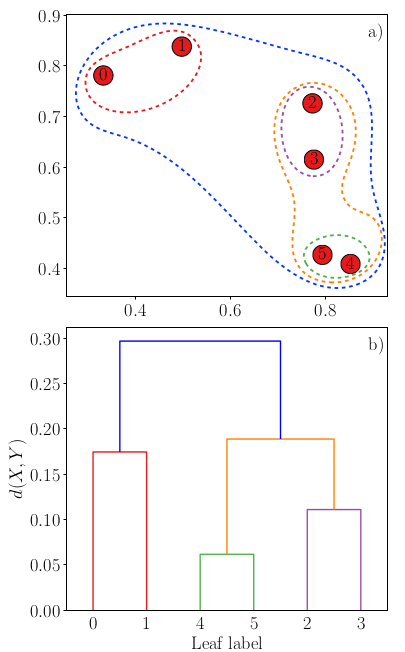
\includegraphics[width=0.4\linewidth]{gfx/HierarchicalCLustering}
	\caption{\itshape The merging process generates a hierarchy of clusters that can be visualized in the form of a dendrogram.}
	\label{fig:hierarchicalclustering}
\end{figure}
This hierarchy \ref{fig:hierarchicalclustering} can be useful to analyze the relation between clusters and the subcomponents of individual clusters. Agglomerative methods are usually specified by defining a distance measure between clusters. Different choices of distance result in different clustering algorithms. At each step, the two clusters that are the closest w.r.t. the distance measure are merged until a single cluster is left.

\begin{mybox}{Agglomerative clustering algorithm}
	\begin{enumerate}
		\item Initialize each point to its own cluster.
		\item Given a set of $K$ clusters $X_1,X_2,\dots,X_K$, merge clusters until one cluster is left ($K=1$):
		\begin{enumerate}
			\item Find the closest pair of clusters $(X_i,X_j)$:
			\bse 
			(i,j)=\arg \min_{i^\prime,j^\prime} d(X_{i^\prime},X_{j^\prime} )
			\ese 
			\item Merge the pair. Update. $K\leftarrow K-1$.
		\end{enumerate}
	\end{enumerate}
\end{mybox}
The most popular distances used in agglomerative methods, often called \emph{linkage methods}
\begin{enumerate}
	\item Single-linkage: the distance between clusters $i$ and $j$ is defined as the minimum distance between two elements of the different clusters
\be
\label{eq:ClusterPracticalHierarchicalSinglelinkage}
d(X_i,X_j) = \min_{\mx_i \in X_i,\mx_j \in X_j} \norm{\mx_i-\mx_j}_2. 
\ee 
\item Complete linkage: the distance between clusters $i$ and $j$ is defined as the maximum distance between two elements of the different clusters
\be 
\label{eq:ClusterPracticalHierarchicalCompleteLinkage}
d(X_i,X_j) = \max_{\mx_i \in X_i,\mx_j\in X_j} \norm{\mx_i-\mx_j}_2.
\ee 
\item Average linkage: average distance between points of different clusters
\be 
\label{eq:ClusterPracticalHierarchicalAverageLinkage}
d(X_i,X_j) = \frac{1}{\abs{X_i}\cdot \abs{X_j}} \sum_{\mx_i \in X_i,\mx_j\in X_j} \norm{\mx_i-\mx_j}_2.
\ee 
\item Ward's linkage: This distance measure is analogous to the $K$-means method as it seeks to minimize the total inertia. The distance measure is the ’error squared’ before and after merging which simplifies to
\be 
\label{eq:ClusterPracticalHierarchicalWardsLinkage}
d(X_i,X_j) = \frac{\abs{X_i} \abs{X_j}}{\abs{X_i \cup X_j}} (\mathbf{μ}_i-\mathbf{μ}_j)^2, 
\ee 
where $\mathbf{μ}_j$ is the centre of cluster $j$.
\end{enumerate}
A common drawback of hierarchical methods is that they do not scale well: At every step, a distance matrix between all clusters must be updated/computed. This leads to a complexity of $\mO(N^2)$, i.e. the method is suitable for small to medium-size datasets.

\subsubsection{Density-based (DB) clustering}
\label{subsubsec:clusterPracticalDBSCAN}
Density clustering makes the intuitive assumption that clusters are defined by regions of space with higher density of data points. Data points that constitute noise or that are outliers are expected to form regions of low density. The method is also suitable for large-scale applications.\\
The core assumption of DB clustering is that a \emph{relative} local density estimation of the data is possible. In other words, it is possible to order points according to their densities. Density estimates are usually accurate for low-dimensional data but become unreliable for high-dimensional data due to large sampling noise.\\
\\
	Consider a set of $N$ data points $X\equiv \{\mx_n\}^N_{n=1}$. Define the $\epsilon$-neighbourhood of point $\mx_n$ 
\be 
N_{\epsilon} (\mx_n) = \{\mx \in X| \md(\mx,\mx_n) < \epsilon \}.
\ee 
$N_{\epsilon}(\mx_n)$ are the data points that are at a distance smaller than $\epsilon$ from $\mx_n$, $\md(\cdot,\cdot)$ is the Euclidean metric. $N_{\epsilon}(\mx_n)$ can be seen as a crude estimate of local density. $\mx_n$ is considered to be a \emph{core-point} if at least \textbf{minPts} are in its $\epsilon$-neighbourhood. \textbf{minPts} is a free parameter of the algorithm that sets the scale of the size of the smallest cluster one should expect. Finally, a point $\mx_i$ is said to be \emph{density-reachable} if it is in the $\epsilon$-neighbourhood of a \emph{core-point}.
\begin{mybox}{DBSCAN algorithm}
\begin{enumerate}
	\item[$\rightarrow$] Until all points in $X$ have been visited; \textbf{do}
	\begin{enumerate}
		\item Pick a point $\mx_i$ that has not been visited
		\item Mark $\mx_i$ as a visited point
		\item If $\mx_i$ is a core point; \textbf{then}
		\begin{enumerate}
			\item Find the set $C$ of all points that are \emph{density reachable} from $\mx_i$.
			\item $C$ now forms a cluster. Mark all points within that cluster as being visited.
		\end{enumerate}
	\end{enumerate}
	\item[$\rightarrow$] Return the cluster assignments $C_1,\dots,C_k$, with $k$ the number of clusters. Points that have not been assigned to a cluster are considered noise or outliers.
\end{enumerate}
\end{mybox}
DBSCAN is very efficient with a $\mO(N\log N)$.

\subsection{Clustering and Latent Variables via the Gaussian Mixture Models}
\label{subsec:clusterConcepts}
Here we collect important concepts of unsupervised learning and showcase them via GMM.
\subsubsection{Important concepts in unsupervised learning}
\label{subsubsec:clusterConceptsCollection}

\begin{mybox}{Important concepts in unsupervised learning}
	\label{subsubsec:clusterConceptsCollectionImportant}
\begin{enumerate}
\item It is often useful to think of the visible correlations between features in the data as resulting from hidden or latent variables.
\item We will often posit a generative model that encodes the structure we think exists in the data and then find the parameters that maximize the likelihood of the observed data.
\item Often we will not be able to directly estimate the MLE, and will have to instead look for a computationally efficient way to find a local minimum of the likelihood.
\end{enumerate}
\end{mybox}
A central concept in many unsupervised learning techniques is the idea of a latent or hidden variable. Even though latent variables are not directly observable, they still influence the visible structure of the data. 
\begin{example}
In the context of clustering we can think of the cluster identity of each datapoint (i.e. which cluster does a datapoint belong to) as a latent variable.
\end{example}
The latent variables in our data (cluster identity) are a way of representing and abstracting the correlations between datapoints.\\

\begin{mybox}{Clustering}
We can think of clustering as an algorithm to learn the most probable value of a latent variable (cluster identity) associated with each datapoint.
\end{mybox}
 Calculating these latent variables requires additional assumptions about the structure of our dataset. Like all unsupervised learning algorithms, in clustering we must make an assumption about the underlying probability distribution from which the data was generated. Our model for how the data is generated is called the \emph{generative model}. In clustering, we assume that data points are assigned a cluster, with each cluster characterized by some \emph{cluster-specific} probability distribution  (e.g. Gaussian with some mean and variance that charaterizes the cluster). We then specify a procedure for finding the value of the latent variable. This is often done by choosing the values of the latent variable that minimize some cost function.\\
 \\
 One common choice for a class of cost functions for many unsupervised learning problems is MLE \ref{subsubsec:bayesEstMLE}. In MLE, we choose the values of the latent variables that maximize the likelihood of the observed data under our generative model (i.e. maximize the probability of getting the observed dataset under our generative model).
 
 
 
 
 
 
 
 \begin{mybox}{Cluster validation}
 	\label{subsubsec:clusterConceptsValidation}
 	\emph{Cluster validation} describes the procedure of verifying whether the obtained labels are ’valid’, which is usually done by visual inspection. That is, the data is represented in a low-dimensional space and the cluster labels obtained are visually inspected to make sure that different labels organize into distinct ’blobs’. This is particularly difficult for high-dimensional data, cf. \ref{subsec:clusterHighD}.
 \end{mybox}
 
 
 
 
\subsubsection{Concepts visualized via the Gaussian Mixture Model (GMM)}
\label{subsubsec:clusterConceptsGMM}
Gaussian Mixture Models are a generative model often used in the context of clustering. In GMM, points are drawn from one of $K$ Gaussians, each with its own mean $\mathbf{μ}_k$ and covariance matrix $\Sigma_k$,
\be 
\label{eq:clusterGMMGaussian}
\mathcal{N}(\mx |\mathbf{μ},\mS) \sim \exp \left[-\half (\mx -\mathbf{μ}) \mS^{-1} (\mx-\mathbf{μ})^T\right].
\ee 
Let us denote the probability that a point is drawn from mixture $k$ by $\pi_k$. Then the probability of generating a point $\mx$ in a GMM is given by
\bse 
p(\mx | \{\mm_k,\mS_k,\pi_k \})= \sum_{k=1}^K \mathcal{N}(\mx |\mm_k,\mS_k) \pi_k.
\ese 
Given a dataset $\mX=\{\mx_1,\dots,\mx_N\}$, we can write the likelihood of the dataset as
\bse 
p(\mX | \{\mm_k,\mS_k,\pi_k\}) = \prod_{i=1}^N p(\mx_i| \{\mm_k,\mS_k,\pi_k \} ).
\ese 
For future reference, let us denote the set of parameters (of $K$ Gaussians in the model) $\{\mm_k,\mS_k,\pi_k\}$ by $\mt$.\\
\\
We will now go through this model exemplifying the important concepts lined out in \ref{subsubsec:clusterConceptsCollectionImportant} in the exact same steps to give an example of these.
\begin{enumerate} 
	\item 
To see how we can use GMM and MLE to perform clustering, we introduce discrete binary $K$-dimensional latent variables $\mathbf{z}$ for each data point $\mx$ whose $k$-th component is $1$ if point $\mx$ was generated from the $k$-th Gaussian and zero otherwise (i.e. one-hot variables).
For instance, if we were considering a Gaussian mixture with $K=3$, we would have three possible values for $\mathbf{z}\equiv (z_1,z_2,z_3): (1,0,0),(0,1,0)$ and $(0,0,1)$. We cannot directly observe the variable $\mathbf{z}$. It is a latent variable that encodes the cluster identity of point $\mx$. Let us also denote all the $N$ latent variables corresponding to a dataset $\mX$ by $\mathbf{Z}$.
\item 
Viewing the GMM as a generative model, we can write the probability $p(\mx |\mathbf{z})$ of observing a data point $\mx$ given $\mathbf{z}$ as\footnote{Note that the notation with $;$ is something we have seen in \ref{eq:infoMutualInfo}, it describes a conditional dependence and makes a distinction between data and parameters.}
\bse 
p(\mx | \mathbf{z}; \{ \mm_k,\mS_k\} ) = \prod_{k=1}^K \mathcal{N}(\mx |\mm_k,\mS_k)^{z_k}
\ese 
as well as the probability of observing a given value of latent variable
\bse 
p(\mathbf{z}| \{\pi_k\}) = \prod_{k=1}^K \pi^{z_k}_k.
\ese 
Using Bayes' rule \ref{eq:bayesrule}, we can write the joint probability of a clustering assignment $\mathbf{z}$ and a data point $\mx$ given the GMM parameter as
\bse 
p(\mx ,\mathbf{z};\mt) = p(\mx| \mathbf{z}; \{\mm_k,\mS_k\} ) p(\mathbf{z}|\{\pi_k\}).
\ese 
Using Bayes' again we find the conditional probability of the data point $\mx$ being in the $k$-th cluster, $\gamma(z_k)$, given model parameters $ \theta$ as 
\be 
\label{eq:clusterConceptsGMMresponsibility}
\gamma(z_k)\equiv p(z_k=1 | \mx;\theta)= \frac{\pi_k \mathcal{N}(\mx|\mu_k,\Sigma_k)}{\sum_{j=1}^K \pi_j \mathcal{N}(\mx |\mu_j,\Sigma_j)}.
\ee 
The $\gamma(z_k)$ are often referred to as the \emph{responsibility} that mixture $k$ takes for explaining $\mx$. Just like in our discussion of soft-max classifiers, this can be made into a ’hard-assignment’ by assigning each point to the cluster with the largest probability: $\arg \max_k \gamma(z_k)$ over the responsibilities.\\
\\
The complication is of course that we do not know the parameters $\mt$ of the underlying GMM but instead must also learn them from the dataset $\mX$. Ideally we would do this by choosing the parameters that maximize the likelihood of the data
\bse 
\hat{\mt} = \arg \max_{\mt} \log p(\mX|\mt).
\ese 
Once we know the MLEs $\hat{\mt}$, we could use \ref{eq:clusterConceptsGMMresponsibility} to calculate the optimal hard cluster assignment $\arg \max_k \hat{\gamma}(z_k)$ where $\hat{\gamma}(z_k) =p(z_k=1|\mx;\hat{\mt})$.

\item It is almost impossible to find the global maximum of the likelihood function. Instead, we must settle for a local maximum. One approach to finding a local maximum of the likelihood is to use a method like SGD \ref{subsubsec:gdSGD} on the negative log-likelihood (i.e. the cost function \ref{eq:bayesErrorFct}), or expectation minimization \ref{subsec:varMFTEM}.
\end{enumerate}


\subsection{Clustering in high dimensions}
\label{subsec:clusterHighD}
One major problem that is aggravated in high-dimensions is the generic accumulation of noise due to random measurement error for each feature. This in turn leads to increased errors for pairwise similarity and distance measures and thus tends to ’blur’ distances between data points.\\
\\
In order to perform clustering on high-dimensional data, it is often useful to denoise the data before proceeding using a standard clustering method such as $K$-means \ref{subsubsec:clusterPracticalKmeans}. 
For example, PCA \ref{subsec:dimRedPCA} can be used to denoise the data by projecting the original $N$ dimensions onto $n < N$ (i.e. $20n\approx N$) with the largest principal components. The resulting features can then be used to construct a Euclidean distance matrix, which in turn can be used by $t$-SNE \ref{subsec:dimRedTSNE} to compute the embedding that is presented. Using $t$-SNE directly on original data leads to a ’blurring’ of the clusters.\\
However, simple feature selection or feature denoising (using PCA for instance) can sometimes be insufficient for learning clusters due to the presence of large variations in the signal and noise of the features that are relevant for identifying the underlying clusters.

\subsubsection{Cluster validation in high dimensions}
For high-dimensional data, cluster validation \ref{subsubsec:clusterConceptsValidation} is done by performing dimensional reduction \ref{sec:dimRed}. However, this can lead to the appearance of spurious clusters since dimensional reduction inevitably loses information about the original data, i.e. use methods with care.\\
Perhaps one of the most intuitive ways of defining a good clustering is by measuring how well the clusters generalizes. Clustering methods based on leveraging powerful classifiers to measure the generalization errors of the \href{https://pypi.org/project/hal-x/}{cluster} could be promising.


\subsection{Practical considerations of clustering methods - when do we use which method ?}
When tuning a clustering method it is important to understand what the implicit assumption of the clustering method are. For instance, methods based on density (local information), will typically fare well at clustering topological datasets since points are connected from neighbour to neighbour. At the same time, methods based on long-distance information ($𝐾$-means for instance), will typically perform poorly in such instances. Density-based methods will, however, have more difficulty at dealing with datasets with large fluctuations in the density distribution of the dataset (3rd row). Another drawback of density based methods is that they do not generalize well to high-dimensional space due to large sampling noise in the density estimates.








\section{Variational Methods and Mean-Field Theory (MFT)}
\label{sec:varMFT}
\subsection{Variational methods introduction}
\label{subsec:varMFTconcept}
A common thread in many unsupervised learning tasks is accurately representing the underlying probability distribution from which a dataset is drawn. When dealing with complicated probability distributions, it is often much easier to learn the \emph{relative weights} of different states or data points (ratio of probabilities), than \emph{absolute} probabilities. 
\begin{example}
	This is the case for statistical physics, where the whole partition function drops out in ratios of cumulants. 
\end{example}
One approach to solve for partition functons is to use Monte-Carlo based methods to draw samples from the underlying distribution (this can be done knowing only the relative probabilities) and then use these samples to numerically estimate the partition function. This is the philosophy behind powerful methods such as Markov Chain Monte Carlo (MCMC).\\
\\
An alternative approach are via variational methods, an example of which is Mean-Field Theory in statistical physics. We use this in the following to explore the concepts of Variational Methods and visualize them on the Ising model.



\subsection{Variational mean-field theory via Ising model}

\subsubsection{Important concepts of MFT}
\label{subsubsec:varMFTconcepts}
\begin{mybox}{Idea variational method}
The alternative approach is to approximate the probability distribution $p(\mx)$ and partition function using a \emph{variational distribution} $q(\mx;\theta_q)$ whose partition function we can calculate exactly. The variational parameters $\theta_q$ are chosen to make the variational distribution as close to the true distribution as possible, this is where the name ’variational distribution’ comes from, because we vary the parameters $\theta_q$.\\
MFT can be naturally understood as a procedure for approximating the true distribution of the system by a factorized distribution.
\end{mybox}
Variational MFT is a systematic way for constructing such an approximate distribution $q(\mx;\theta_q)$.\\
Even though MFT is not exact, it can often yield qualitatively and even quantitatively precise predictions (especially in high dimensions). The discrepancy between the true physics and MFT predictions stems from he fact that the variational distribution $q$ we chose cannot capture correlations. These correlations become less and less important in higher dimensions and the MFT ansatz becomes more accurate.\\
We emphasize that the failure of any particular variational ansatz does not compromise the usefulness of the approach. In some cases, one can consider changing the variational ansatz to improve the predictive properties of the corresponding variational MFT.
\subsubsection{On the example of the Ising model}
\label{subsubsec:varMFTising}
Here we discuss the ideas given in \ref{subsubsec:varMFTconcepts} on the example of the Ising model.\\
The probability of finding the Ising system in a given spin configuration at temperature $\beta^{-1}$ is given by
\bse 
p(\mathbf{s} |\beta,\mathbf{J}) = \frac{1}{Z_p(\mathbf{J})} e^{-\beta E(\mathbf{s},\mathbf{J}) }.
\ese 
Even though the true probability distribution $p(\mathbf{s}|\beta,\mathbf{J})$ may be a very complicated object, we can still make progress by approximating $p(\mathbf{s}|\beta,\mathbf{J})$ by a \emph{variational distribution}
$q(\mathbf{s},\mt)$ which captures the essential features of interest, with $\mt$ some parameters that define our variational ansatz.\\
The main idea is to choose parameters that minimize the difference between the variational free-energy $F_q(\mathbf{J},\mt)$ and the true free-energy $F_p(\mathbf{J}|\beta)$. This is
\bse 
F_q(\mathbf{J},\mt) = F_p(\mathbf{J},\beta) + D_{KL}(q||p),
\ese 
with the KL-divergence \ref{eq:infoKLdivergence}. Its properties show us that the variational free-energy is always larger than the true free energy $F_q (\mathbf{J},\mt) \geq F_p(\mathbf{J})$,with equality if and only if $q=p$ (the latter inequality is known as Gibbs inequality). They also show us that finding the best variational free-energy is equivalent to minimizing the KL divergence.
\\
\\
One starts the MFT by making an ansatz for the variational distribution $q(\mathbf{s},\mt)$ which is here chosen such that all spins are independent, i.e. ignoring spin correlations. This gives us the free energy via the partition function (which became analytically solvable), the former of which we then try to minimize w.r.t. the variational parameters $\mt$. One obtains the mean-field equations for the Ising model
\begin{align}
	m_i &= \expval{s_i}_q = \sum_{s_i=\pm 1} s_i \frac{e^{\theta_i s_i}}{2 \cosh \theta_i} = \tanh(\theta_i),\label{eq:varMFTIsing1}\\
	\theta_i &= \beta \sum_j J_{ij} m_j(\theta_j) + h_i \label{eq:varMFTIsing2}.
\end{align}
To find a solution to these equations, one method is to iterate through and update each $\theta_i$, once at a time, in an asynchronous fashion. The iterative procedure to find the solutions to \ref{eq:varMFTIsing2} is given by the following.\\
We start by initializing our variational parameters to some $\mt^{(0)}$ and repeat the following two steps until convergence:
\begin{enumerate}
	\item \emph{Expectation}:\\
	Given a set of assignments at iteration $t$, $\mt^{(t)}$, calculate the corresponding magnetizations $\mathbf{m}^{(t)}$ using \ref{eq:varMFTIsing1}.
	\item \emph{Maximization}:\\
	Given a set of magnetizations $m_t$, find new assignments $\theta^{(t+1)}$ which minimize the variational free energy $F_q$. From \ref{eq:varMFTIsing2}, this is just
	\bse 
	\theta^{(t+1)}_i = \beta \sum_j J_{ij} m^{(t)}_j +h_i.
	\ese 
\end{enumerate}













 
\subsection{Expectation Maximization (EM)}
\label{subsec:varMFTEM}
Expectation-Maximization (EM) is a practical way to perform maximum likelihood estimation (MLE) even when some of the data is hidden (i.e in the presence of latent or hidden variables)\\
EM is a general method that can be derived for any latent (hidden) variable model using a variational procedure. We will focus on latent variable models where some of the variables are hidden and cannot be directly observed. This often makes MLE \ref{subsubsec:bayesEstMLE} difficult to implement. EM gets around this difficulty by using an iterative two-step procedure closely related to variational free-energy based approximation schemes in stat. phys.
\subsubsection{EM in a nutshell - mathematical}
\label{subsubsec:varMFTEMmath}
To set the stage, let $\mx$ be the set of visible variables we can directly observe and $\mathbf{z}$ be the set of latent or hidden variables that we cannot directly observe. Denote the underlying probability distribution from which $\mx$ and $\mathbf{z}$ are drawn by $p(\mathbf{z},\mx |\mt)$, with $\mt$ representing all relevant parameters. Given a dataset $\mx$, we wish to find the MLE of the parameters $\mt$ that maximizes the probability of the observed data.\\
As in variational MFT \ref{subsec:varMFTconcept}, we view $\mt$ as variational parameters chosen to maximize the log-likelihood $L(\mt)=\expval{\log p(\mx|\mt)}_{P_{\mx}}$, where the expectation is taken with respect to the marginal distributions of $\mx$.
\begin{mybox}{EM in a nutshell}
EM is a powerful approach for finding local minima in latent variable models using an iterative procedure. Given an initial guess for the parameters $\theta^{(0)}$, the EM algorithm iteratively generates new estimates for the parameters $\theta^{(1)},\theta^{(2)},\dots$ Importantly, the likelihood is guaranteed to be non-decreasing under these iterations and hence EM converges to a local maximum of the likelihood. This is formulated in the following:
\begin{enumerate}
\item \emph{Expectation step (E step)}:\\
Given the known values of observed variable $\mx$ and the current estimate of parameter $\mt_{t-1}$, find the probability distribution of the latent variable $\mathbf{z}$:
\be 
\label{eq:varMFTEM1}
q_{t-1}(\mathbf{z}) = p(\mathbf{z}|\mt^{(t-1)}, \mx).
\ee 
\item \emph{Maximization step (M step)}:\\
Re-estimate the parameter $\mt^{(t)}$ to be those with with maximum likelihood, assuming $q_{t-1}(\mathbf{z})$ found in the previous step is the true distribution of hidden variable $\mathbf{z}$:
\be 
\label{eq:varMFTEM2}
\mt_t = \arg \max_{\mt} \expval{\log p(\mathbf{z},\mx |\mt)}_{q_{t-1}}.
\ee 
\end{enumerate}
It was shown that each EM iteration increases the true log-likelihood $L(\mt)$, or at worst leaves it unchanged. In most models, this iteration procedure converges to a \emph{local maximum} of $L(\mt)$.
\end{mybox}

\begin{mybox}{EM in application}
	The E-M algorithm often approximates the MLE even in the presence of latent (hidden variables). Like with most optimization methods for non-concave functions, E-M only guarantees convergence to a local maximum of the objective function. For this reason, its performance can be boosted by running the EM procedure starting with multiple initial parameters.
\end{mybox}
\subsubsection{EM via statistical physics}
\label{subsubsec:varMFTEMphys}
Recall that our goal is to maximize the log-likelihood $L(\mt)$. With data $\mathbf{z}$ missing, we surely cannot just maximize $L(\mt)$ directly since parameter $\mt$ might couple both $\mathbf{z}$ and $\mx$. EM circumvents this by optimizing another objective function, $F_q(\mt)$, constructed based on estimates of the hidden variable distribution $q(\mathbf{z}|\mx)$. Indeed, the function optimized is none other than the \emph{variational free energy}, encountered in \ref{subsubsec:varMFTising}.\\
Then, the maximization step (M-step) in the algorithm in  \ref{eq:varMFTEM2} is equivalent to minimizing the variational free-energy $F_q(\mt)$. Surprisingly, the expectation step (E-step) can also be viewed as the optimization of this variational free-energy. Concretely, one can show that the distribution of hidden variables $\mathbf{z}$ given the observed variable $\mx$ and the current estimate of parameter $\mt$, \ref{eq:varMFTEM1}, is the \emph{unique} probability $q(\mathbf{z})$ that minimizes $F_q(\mt)$.\\
\begin{mybox}{EM algorithm in physics language}
	We can re-write EM as follows:
	\begin{enumerate}
		\item \emph{Expectation Step:}\\
		Construct the approximating probability distribution of unobserved $\mathbf{z}$ given the values of observed variable $\mx$ and parameter estimate $\mt^{(t-1)}$:
		\be 
		q_{t-1}(\mathbf{z}) = \arg \min_q F_q (\mt^{(t-1)}).
		\ee 
		\item \emph{Maximization step:}\\
		Fix $q$, update the variational parameters
		\be 
		\mt^{(t)} = \arg \max_{\mt} -F_{q_{t-1}} (\mt).
		\ee 
	\end{enumerate}
\end{mybox}
\begin{mybox}{Summary Em physics language}
	EM implements ML estimation \ref{subsubsec:bayesEstMLE} even with missing or hidden variables through optimizing a lower bound of the true log-likelihood. In stat. phys., this is reminiscent of optimizing a variational free-energy which is a lower bound of true free-energy due to Gibbs inequality. The E-step can be seen as representing the unobserved variable $\mathbf{z}$ by a probability distribution $q(\mathbf{z})$. This probability is used to construct an alternative objective function $-F_q(\mt)$, which is then maximized w.r.t. $\mt$ in the M-step. By construction, maximizing the negative variational free-energy is equivalent to doing ML estimation on the joint data (i.e. bot observed and unobserved). The name ’M-step’ is intuitive since the parameters $ \mt$ are found by maximizing $-F_q(\mt)$. The name ’E-step’ comes from the fact that one usually doesn' t need to construct the probability of missing data explicitly, but rather need only compute the ’expected’ sufficient statistics over these data.
\end{mybox}
In many cases, implementation of EM is guaranteed to increase the likelihood monotonically, which could be a perk during debugging.\\
For a comparison between EM and statistical physics see \ref{fig:analogyemstatphys}.

\begin{figure}[h!]
	\centering
	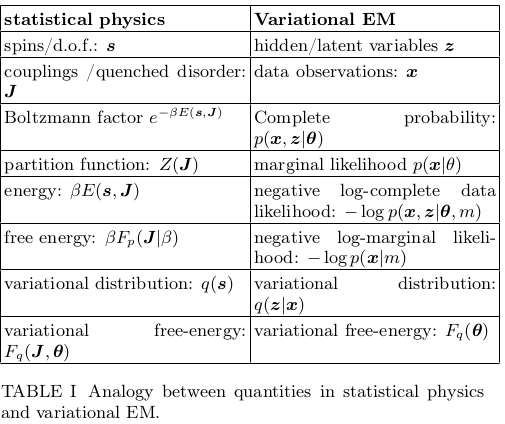
\includegraphics[width=0.7\linewidth]{gfx/AnalogyEMstatphys}
	\caption{}
	\label{fig:analogyemstatphys}
\end{figure}















